\documentclass[../main/main.tex]{subfiles}
\begin{document}

\chapter{Curvature}

%%%%%%%%%% LECTURE 8.III %%%%%%%%%%

\section{Curvature}
\textsf{Carroll, sec. 3.6}\\

The aim of this section is to give an answer to the following question: is there any \emph{intrinsic} way to characterize a ``honest''gravitational field? That is, a metric $g_{\mu\nu}(x)$ for which there does not exist any inertial frame $\hat x^\alpha$ in which
\[\de s^2=g_{\mu\nu}(x)\de x^\mu\de x^\nu=\eta_{\mu\nu}\de\hat x^\mu\de\hat x^\nu\qquad\text{and}\qquad\hchris\mu\rho\sigma\equiv0\]

Let us first observe that a property of Minkowski space is that the parallel transport between two points does not depend on the path. This is obvious in flat (inertial) coordinates, in which $\hchris\mu\rho\sigma\equiv0$
\[\cder{\hat V^\mu}\lambda\equiv\der{\hat V^\mu}\lambda=0\quad\Leftrightarrow\qquad\hat V^\mu(\lambda)=\text{constant}\]
which implies
\[\hat V^\mu_B\vert_{\gamma_1}=\hat V_A^\mu=\hat V^\mu_B\vert_{\gamma_2}\]
and
\[V^\mu_B\vert_{\gamma_1}= V^\mu_B\vert_{\gamma_2}\qquad\text{in any other coordinates }x^\mu\]
%
\begin{figure}[H]
\centering
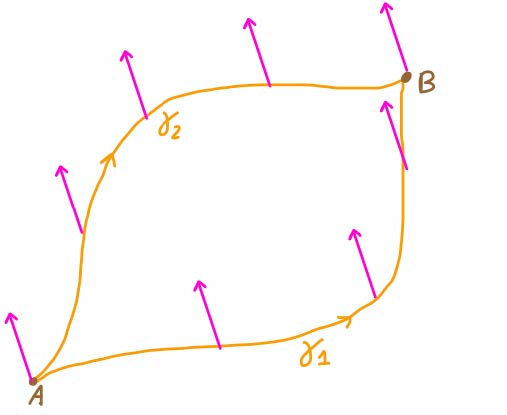
\includegraphics[width=6cm]{../img/curv-path-comm.jpg}
\end{figure}

For a more generic metric, we generally have $V^\mu(\lambda_{\text{fin}})\neq V^\mu(\lambda_{\text{in}})$. Indeed
\[\der{V^\mu(s)}s=-\chris\mu\nu\rho(X(s))V^\nu(s)\dot X^\rho(s)\]
which implies
\[V^\mu(s+\delta s)=V^\mu(s)=\chris\mu\nu\rho(X(s))V^\nu(s)\overbrace{\dot X^\rho(s)\delta s}^{\delta X^\rho(s)}+\dots\]
and then the infinitesimal change of $V^\mu$ parallely transported along $\delta X^\mu$ is given by
\[\delta V^\mu=-\chris\mu\nu\rho(x)V^\nu\delta X^\rho\]
%
\begin{figure}[H]
\centering
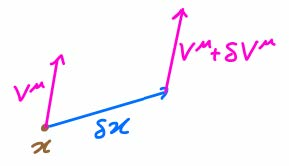
\includegraphics[width=4cm]{../img/curv-V-parall-trasp.jpg}
\end{figure}

Consider now two independent infinitesimal displacements $\delta_1X^\mu$, $\delta_2X^\mu$:
%
\begin{figure}[H]
\centering
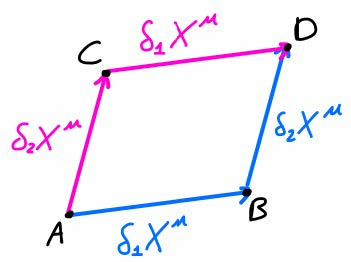
\includegraphics[width=5cm]{../img/curv-2-infinit-displ.jpg}
\end{figure}
in formulas we have (in the second step we used $x_B=x_A+\delta_1X$)
\begin{align*}
V_D^\mu\vert_{1-2}
&=V_B^\mu-\chris\mu\nu\rho(x_B)V_B^\nu\delta_2X^\rho\\
&=V_A^\mu-\chris\mu\nu\rho(x_A)V_A^\nu\delta_1X^\rho-\chris\mu\nu\rho(x_A)V_A^\nu\delta_2X^\rho\\
&\quad-\partial_\sigma\chris\mu\nu\rho(x_A)V_A^\nu\delta_1X^\sigma\delta_2X^\rho+\chris\mu\nu\rho(x_A)\chris\nu\alpha\sigma(x_A)V_A^\alpha\delta_1X^\sigma\delta_2X^\rho\\
V_D^\mu\vert_{2-1}&=(\text{the same with }1\leftrightarrow)
\end{align*}
Then $V_D^\mu\vert_{1-2}-V_D^\mu\vert_{2-1}=-\curv\mu\nu\rho\sigma(x_A)V_A^\nu\delta_1X^\rho\delta_2X^\sigma$ where we defined the \textbf{Riemann curvature}:
\begin{equation}\label{eqn:Riemann-curvature}\boxed{
\curv\mu\nu\rho\sigma\equiv\partial_\rho\chris\mu\nu\sigma-\partial_\sigma\chris\mu\nu\rho+\chris\mu\alpha\rho\chris\alpha\nu\sigma-\chris\mu\alpha\sigma\chris\alpha\nu\rho
}\end{equation}
Notice that this is a tensor. For any vector field $V^\mu(x)$ we have
\[[\nabla_\rho,\nabla_\sigma]V^\mu\equiv(\nabla_\rho\nabla_\sigma-\nabla_\sigma\nabla_\rho)V^\mu=\curv\mu\nu\rho\sigma V^\nu\]
(on the l.h.s. of the previous identity we omitted the factor $-\tens T\nu{\rho\sigma}\nabla_\nu V^\mu$ with $\tens T\nu{\rho\sigma}=2\Gamma^\nu_{[\rho\sigma]}$ since it vanishes). 

For more generic tensors $\tens T{\mu\dots}{\nu\dots}$ we have
\begin{align*}
[\nabla_\rho,\nabla_\sigma]\tens T{\mu\dots}{\nu\dots}
&=\curv\mu\tau\rho\sigma \tens T{\tau\dots}{\nu\dots}+(\text{similar action on \emph{upper} indices})\\
&\quad-\curv\tau\nu\rho\sigma \tens T{\mu\dots}{\tau\dots}+(\text{similar action on \emph{lower} indices})
\end{align*}
Note also that $[\nabla_\mu,\nabla_\nu]\phi=0$ for any scalar field. 

Note that for $\de s^2=\eta_{\alpha\beta}\de\hat x^\alpha\de\hat x^\beta$ we clearly have $\hcurv\mu\nu\rho\sigma\equiv0$, hence $\curv\mu\nu\rho\sigma\equiv0$ in any other coordinate system $x^\mu$ ( even if $\chris\mu\nu\rho\neq0$). Viceversa, if $\curv\mu\nu\rho\sigma\equiv0$ then one can find\footnote{See, for instance, Carroll pag. 124} a local coordinate system $\hat x^\alpha$ in which $\de s^2=\hat\eta_{\alpha\beta}\de\hat x^\alpha\de\hat x^\beta$. 

On the other hand, if $\curv\mu\nu\rho\sigma\not\equiv$ there do not exist inertial coordinates. Hence we arrived to the following important result:
\begin{equation}\boxed{\begin{split}
\text{spacetime is \emph{flat} (and locally like Mink)}\quad&\Leftrightarrow\quad\curv\mu\nu\rho\sigma\equiv0\\
\text{spacetime is \emph{curved}}\quad&\Leftrightarrow\quad\curv\mu\nu\rho\sigma\not\equiv0
\end{split}}\end{equation}

Note that (if $[x^\mu]=L$) the curvature has dimension $[\curv\mu\nu\rho\sigma]=(\text{length})^{-2}$. In particular, $(\curv\mu\nu\rho\sigma)^{-1/2}$ provides an estimate of the length scale $L$ above which the space-time cannot be approximated by the flat one. This also set the scale below which the EEP holds. 

Previous claim can be made precise by introducing \emph{normal} coordinates. 

\subsection{Geodesic (or Riemann) normal coordinates}

At any point $p$, choose orthonormal frame $e_\alpha=e_\alpha^\mu\partial_\mu$. Any $V\in T_pM$ can be decomposed as $V=\hat x^\alpha e_\alpha$
%
\begin{figure}[H]
\centering
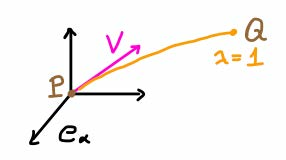
\includegraphics[width=4cm]{../img/curv-norm-coord.jpg}
\end{figure}
\noindent
Throw a geodesic with affine parameter $\lambda$ ($[\lambda]=1$) such that $\der{X^\mu}\de\lambda\vert_{\lambda=0}=V^\mu$. The value $\lambda-1$ identifies a point $q$, hence assign coordinates $\hat x^\alpha$ to $q$. In this way we obtained a defined coordinate system $\hat X^\alpha$ in a small enough neighbourhood of $\hat x^\alpha=0$. In this coordinate system
\begin{equation}\boxed{
\hchris\alpha\beta\gamma\vert_p=0\qquad\hat g_{\alpha\beta}(\hat x)=\eta_{\alpha\beta}-\frac13\hat R_{\alpha\gamma\beta\delta}\hat x^\gamma\hat x^\delta+\dots
}\end{equation}
and $\hat g_{\alpha\beta}=\eta_{\alpha\beta}+O\p{\frac{\hat x^2}{L^2}}$ with $L^2\simeq(\text{Riem})^{-2}$ as claimed above and $\hat x^2$ which approximates the proper ``distance'' from $p$. 

Such construction is the concrete realization of the EEP. The error is given by $\frac{(\text{distance})^2}{L^2}$ with $L^2\sim(\text{Riem})^{-1}$.

%%%%%%%%%%LECTURE 9%%%%%%%%%%%%%%%

\subsection{Properties of the Riemann tensor}

\textsf{Carroll, sec. 3.7}

It is convenient to introduce the tensor 
\[R_{\mu\nu\rho\sigma}:=g_{\mu\tau}\curv\tau\nu\rho\sigma\]
which satisfies following properties:
\begin{subequations}
\begin{align}
&R_{\mu\nu\rho\sigma}=-R_{\mu\nu\sigma\rho}=R_{\mu\nu[\rho\sigma]}\\
&R_{\mu\nu\rho\sigma}=-R_{\nu\mu\rho\sigma}=R_{[\mu\nu]\rho\sigma}\\
&R_{\mu\nu\rho\sigma}=R_{\rho\sigma\mu\nu}\\
&R_{\mu\nu\rho\sigma}+R_{\mu\rho\sigma\nu}+R_{\mu\sigma\nu\rho}=0\hspace{1cm}(\overset{a}\Leftrightarrow\quad R_{\mu[\nu\rho\sigma]}=0)
\end{align}\end{subequations}
In order to prove above properties at any point $p$, we can use any locally inertial frame $\hat x^\alpha$:
\[\hchris\alpha\beta\gamma=0\quad\Leftrightarrow\quad\hat\partial_\alpha\hat g_{\beta\gamma}=0\quad\Leftrightarrow\quad\hat\partial_\alpha\hat g^{\beta\gamma}=0\qquad(\text{at }p)\]
Then, at $p$:
\begin{align*}
\hat R_{\alpha\beta\gamma\delta}
&=\hat g_{\alpha\lambda}(\hat\partial_\gamma\hchris\lambda\beta\delta-\hat\partial_\delta\hchris\lambda\beta\gamma)\hspace{2cm}\\
&=\frac12(\hat\partial_\gamma\hat\partial_\beta\hat g_{\alpha\delta}-\hat\partial_\delta\hat\partial_\beta\hat g_{\alpha\gamma}-\hat\partial_\gamma\hat\partial_\alpha\hat g_{\beta\delta}+\hat\partial_\delta\hat\partial_\alpha\hat g_{\beta\gamma}
\end{align*}
In this way one can immediately check properties (a), (b) and (c) and, with slightly more work, (d).

The Riemann tensor obeys also a differential identity, called \textbf{Bianchi identity}:
\begin{equation}\boxed{
\nabla_{[\mu}R_{\nu\rho]\sigma\lambda}=\nabla_{[\mu\vert}R_{\sigma\lambda\vert\nu\rho]}=0
}\end{equation}
One may prove it in local flat coordinates (see Carroll, pag. 128) but it is easier to obtain it from the tautological \textbf{Jacobi identity}:
\[[\nabla_\mu,[\nabla_\nu,\nabla_\rho]]+[\nabla_\nu,[\nabla_\rho,\nabla_\mu]]+[\nabla_\rho,[\nabla_\mu,\nabla_\nu]]=0\]
and applying it to a generic vector field $V^\sigma$:
\begin{align*}
[\nabla_\mu,[\nabla_\nu,\nabla_\rho]]V^\sigma
&=\nabla_\mu(\curv\sigma\tau\nu\rho V^\tau)-[\nabla_\nu,\nabla_\rho]\nabla_\mu V^\sigma\\
&=(\nabla_\mu\curv\sigma\tau\nu\rho)V^\sigma+\underbrace{\curv\sigma\tau\nu\rho\nabla_\mu V^\tau-\curv\sigma\tau\nu\rho\nabla_\mu V^\tau}_{=0}+\curv\tau\mu\nu\rho\nabla_\tau V^\sigma
\end{align*}
Then antisymmetrizing on $\mu\nu\rho$ and using $\curv\tau{[\mu}\nu{\rho]}\equiv0$ one gets the Bianchi identity in the form $\nabla_{[\mu\vert}\curv\tau\sigma{\vert\nu}{\rho]}\equiv0$.

Some important quantities can be obtained through the contraction of indices in the Riemann tensor $\curv\mu\nu\rho\sigma$:
\begin{enumerate}[label=(\alph*)]
\item \textbf{Ricci tensor}:
\begin{equation}\boxed{
 R_{\mu\nu}\equiv\curv\rho\mu\rho\nu
}\end{equation}
Note that
\[ R_{\nu\mu}=\curv\rho\nu\rho\mu={{R_{\rho\mu}}^\rho}_\nu=\curv\rho\mu\rho\nu= R_{\mu\nu}\]
\item\textbf{Scalar curvature}
\begin{equation}\boxed{
 R\equiv g^{\mu\nu}R_{\mu\nu}
}\end{equation}
with $[R]=L^{-2}$
\item\textbf{Einstein tensor}
\begin{equation}\boxed{
 G_{\mu\nu}\equiv R_{\mu\nu}-\frac12g_{\mu\nu}R
}\end{equation}
\end{enumerate}

By contracting the Bianchi identity we get
\begin{align*}
0&=\imet\nu\sigma\imet\mu\lambda(\nabla_\mu R_{\nu\rho\sigma\lambda}+\nabla_\nu R_{\rho\mu\sigma\lambda}+\nabla_\rho R_{\mu\nu\sigma\lambda})\\
&=\nabla^\lambda R_{\rho\lambda}+\nabla^\sigma R_{\sigma\rho}-\nabla_\rho R
\end{align*}
which implies
\begin{equation}\boxed{
\nabla^\mu R_{\mu\nu}=\frac12\nabla_\nu R\qquad\Leftrightarrow\qquad\nabla^\mu G_{\mu\nu}=0
}\end{equation}
Notice that the previous relation for the Einstein tensor will be important in the future. 

\begin{example}[$S^2$ with round metrix]

Consider $S^2$ with a round metric of radius $L$:
\[\de s^2=L^2(\de\theta^2+\sin^2\theta\de\phi^2)\]
i.e.
\[\met\theta\theta=L^2\qquad\met\phi\phi=L^2\sin^2\theta\qquad\met\theta\phi=\met\phi\theta=0\]

The connection is
\begin{align*}
&\chris\theta\phi\phi=-\frac12\imet\theta\theta\pde\theta\met\phi\phi=-\frac12\p{\frac1{L^2}}2L^2\sin\theta\cos\theta=-\sin\theta\cos\theta\\
&\chris\phi\phi\theta=\chris\phi\theta\phi=\frac12\imet\phi\phi\pde\theta\met\phi\phi=\frac1{2L^2\sin^2\theta}2L^2\sin\theta\cos\theta=\cot\theta\\
&\chris\theta\theta\theta=\chris\theta\theta\phi=\chris\phi\phi\phi=0
\end{align*}

The Riemann tensor has only one independent component $R_{\theta\phi\theta\phi}=\met\theta\theta\curv\theta\phi\theta\phi$ where
\[\curv\theta\phi\theta\phi=\pde\theta\chris\theta\phi\phi-\pde\phi\chris\theta\phi\theta+\chris\theta\mu\theta\chris\mu\phi\phi-\chris\theta\mu\phi\chris\mu\phi\theta=\sin^2\theta-\cos^2\theta+\cos^2\theta=\sin^2\theta\]

The Ricci tensor is
\begin{align*}
&R_{\phi\phi}=\sin^2\theta\\
&=R_{\theta\theta}=\curv\phi\theta\phi\theta=\imet\phi\phi R_{\phi\theta\phi\theta}=\imet\phi\phi\met\theta\theta\curv\theta\phi\theta\phi=1
\end{align*}
and so we obtained
\begin{equation}\boxed{
\ricc\mu\nu=\frac1{L^2}\met\mu\nu
}\end{equation}

The scalar curvature is 
\[R=\imet\theta\theta\ricc\theta\theta+\imet\phi\phi\ricc\phi\phi=\frac1{L^2}(1+1)=\frac2{L^2}\]
which is obviously constant because of natural invariance. 

The Einstein tensor is 
\[\eten\mu\nu=\ricc\mu\nu-\frac12\met\mu\nu R=0\]

Can be proved that the Einstein tensor is always zero in two dimension. Use normal coordinates to prove this statement. 

\end{example}

\begin{example}[The evolving universe]
The metric for the evolving universe is
\[\de s^2=-\de t^2+a^2(t)\delta_{ij}\de x^i\de x^j\]
with connection
\[\chris0ij=a\dot a\delta_{ij}\qquad\chris ij0=\chris i0j=\frac{\dot a}a\delta^i_j\]

The Riemann tensor has following components:
\begin{align*}
\curv0i0j&=\pde0\chris0ij-\pde j\chris0i0+\chris0k0\chris kij-\chris0kj\chris ki0\\
&=\der{}t(a\dot a)\delta_{ij}-a\dot a\delta_{kj}\p{\frac{\dot a}a}\delta^k_i=a\dot a\delta_{ij}
\quad\Rightarrow\quad\text{independent components}\\
\curv0ijk&=0-0+\chris0lj\chris lik-\chris0lk\chris lij=0=\chris ijk0\\
\curv ijkl&=\chris i0k\chris0jl-\chris i0l\chris0jk=(\dot a)^2(\delta^i_k\delta_{jl}-\delta^i_l\delta_{jk})
\end{align*}

For the Ricci tensor
\begin{align*}
\ricc00&=\curv i0i0=\imet ij\tcurv0i0j=-\frac1{a^2}\delta^{ij}(a\dot a\delta_{ij})=-3\frac{\ddot a}{a}\\
\ricc ij&=\curv0i0j+\curv kikj=a\ddot a\delta_{ij}+\dot a^2(3\delta_{ij}-\delta_{ij})=(2\dot a^2+a\ddot a)\delta_{ij}\\
\ricc0i&=\curv\mu0\mu i=0
\end{align*}

The scalar curvature is
\[R=\imet00\ricc00+\met ij\ricc ij=3\frac{\ddot a}a+\frac1{a^2}\delta^{ij}[(2\dot a^2+a\ddot a)\delta_{ij}]=6\left[\frac{\ddot a}a+\p{\frac{\dot a}a}^2\right]\]

The Einstein tensor is 
\begin{align*}
\eten00&=-3\frac{\ddot a}a+\frac12\cdot 6\left[\frac{\ddot a}a+\p{\frac{\dot a}a}^2\right]=3\p{\frac{\dot a}a}^2\\
\eten ij&=(2\dot a^2+a\ddot a)\delta_{ij}-3(a\ddot a+\dot a^2)\delta_{ij}=-(\dot a^2+2a\ddot a)\delta_{ij}
\end{align*}

Take for instance the exponential of the de Sitter expansion
\[a(t)=e^{Ht}\qquad H=\frac{\dot a}a\]
Then $\frac{\ddot a}a=H^2$ and this implies
\begin{equation}\boxed{
R=12H^2
}\end{equation}
This implies that $H^{-1}$ (Hubble scale) approximates the radius of curvature and
\begin{equation}\boxed{
\eten\mu\nu=-3H^2\met\mu\nu
}\end{equation}
approximates the empty space-time with positive cosmological constant. 

\end{example}

\section{Geodesic deviation}
\textsf{Carroll, sec. 3.10}

There are various possible normal coordinates (LIFs). For instance, the Fermi normal coordinates constructed around a freely falling observer provide the mathematical realisation of Einstein's freely-falling cabin. 
%
\begin{figure}[H]
\centering
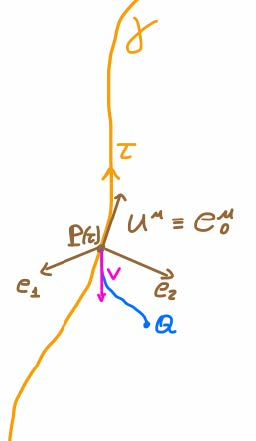
\includegraphics[width=4cm]{../img/Fermi-normal-coord-free.jpg}
\end{figure}
\noindent
In Fermi normal coordinates $\hat x^\alpha=(\hat x^0,\hat x^a)$ with $\hat x^0=\tau$ te connection becomes
\begin{equation}\boxed{
\hchris\alpha\beta\gamma(\tau,\vect 0)\equiv0\quad\Leftrightarrow\quad\hpde\alpha\hmet\beta\gamma\vert_\gamma=0
}\end{equation}
and in components
\begin{equation}\boxed{\begin{split}
\hmet00&=-1-\htcurv0a0b\vert_\gamma\hat x^\alpha\hat x^b+\dots\\
\hmet ab&=\delta_{ab}-\frac13\htcurv abcd\vert_\gamma\hat x^c\hat x^d+\dots\\
\hmet0a&=\frac23\htcurv0bca\vert_\gamma\hat x^b\hat x^c+\dots
\end{split}}\end{equation}

The next question is how can we measure the effect of a non-trivial gravitational field. The answer is given measuring the relative motion of two bodies. 

Let us start from the case of flat space, $\chris\mu\nu\rho\equiv0$, and consider two geodesics $X^\mu(\lambda)$ and $Y^\mu(\lambda)=X^\mu(\lambda)+S^\mu(\lambda)$ for an affine parameter $\lambda$ and with constant relative velocity $U^\mu\equiv\der{X^\mu}\lambda$ and $V^\mu\equiv\der{S^\mu}\lambda$. 
If $V^\mu=0$ we have the following situation:
\begin{figure}[H]
\centering
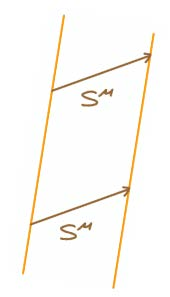
\includegraphics[width=2.5cm]{../img/geodesic-deviation-v0.jpg}
\end{figure}
\noindent
while if $V^\mu\neq$ constant, but $A^\mu\equiv\der{V^\mu}\lambda\equiv0$, we have vanishing relative acceleration:
\begin{figure}[H]
\centering
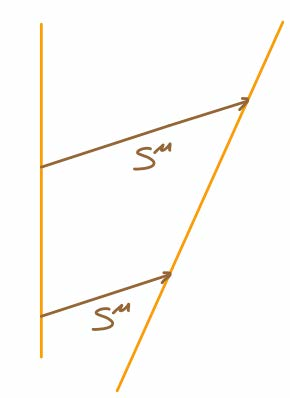
\includegraphics[width=3cm]{../img/geodesic-deviation-vnot0.jpg}
\end{figure}

For general coordinates and metrics the relative distance on nearby geodesics changes in a way dictated by the Riemann tensor. For instance, take two nearby geodesics $X^\mu(\lambda)$ and $Y^\mu(\lambda)=X^\mu(\lambda)+\epsilon S^\mu(\lambda)$ for an affine parameter $\lambda$
\begin{figure}[H]
\centering
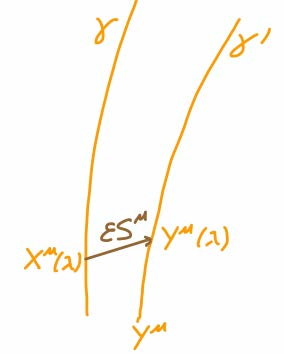
\includegraphics[width=3cm]{../img/geodesic-deviation.jpg}
\end{figure}
\noindent
In order to evaluate the relative acceleration at a point $p\in\gamma$ let us use normal coordinates $\hat x^\alpha$ around it, so that $\hchris\alpha\beta\gamma\vert_p=0$ we have $\frac{\de^2\hat X^\alpha(\lambda)}{\de\lambda^2}\big\vert_p=0$ which implies
\[0=\left[\frac{\de^2\hat Y^\alpha(\lambda)}{\de\lambda^2}+\hchris\alpha\beta\gamma(\hat Y)\der{\hat Y^\beta}\lambda\der{\hat Y^\gamma}\lambda\right]=\epsilon\left[\frac{\de^2\hat S^\alpha}{\de\lambda^2}+\hpde\delta\hchris\alpha\beta\gamma\der{\hat X^\beta}\lambda\der{\hat X^\gamma}\lambda\hat S^\delta\right]\Bigg\vert_p+O(\epsilon^2)\]
which implies
\begin{equation}\label{eqn:geod-deviation-eq1}
\frac{\de^2\hat S^\alpha}{\de\lambda^2}\bigg\vert_p=-\hpde\delta\hchris\alpha\beta\gamma\der{\hat X^\beta}\lambda\der{\hat X^\gamma}\lambda\hat S^\delta\bigg\vert_p
\end{equation}
Then the acceleration is
\begin{align*}
\hat A^\alpha\vert_p
&=\der{\hat V^\alpha}\lambda\big\vert_p
=\left[\der{}\lambda\p{\der{\hat S^\alpha}\lambda+\hchris\alpha\beta\gamma\der{\hat X^\gamma}\lambda\hat S^\beta}\right]\Bigg\vert_p\\
&=\p{\frac{\de^2\hat S^\alpha}{\de\lambda^2}+\hpde\delta\hchris\alpha\beta\gamma\der{\hat X^\delta}\lambda\der{\hat X^\gamma}\lambda\hat S^\beta}\bigg\vert_p
\overset{\eqref{eqn:geod-deviation-eq1}}{=}
\underbrace{\p{\hpde\delta\hchris\alpha\beta\gamma-\hpde\beta\hchris\alpha\gamma\delta}}_{\hcurv\alpha\gamma\delta\beta}\der{\hat X^\delta}\lambda\der{\hat X^\gamma}\lambda\hat S^\beta
\end{align*}
So we obtained that in any coordinate system the geodesic deviation is given by
\begin{equation}\boxed{
A^\mu(\lambda)=\sqcder{S^\mu}\lambda=\curv\mu\nu\rho\sigma(X)\dot X^\nu\dot X^\rho S^\sigma
}\end{equation}
which is called \textbf{geodesic deviation equation}. 

This quantifies the fact that the curvature determines how closely freely falling points accelerate towards or away each other, hence implies the gravitational ``tidal effects'' (for physical coordinates we have independent effects).

\begin{exercise}
Compute the relative acceleration between two nearby (comoving) coordinate observers in an expanding universe. 
\begin{figure}[H]
\centering
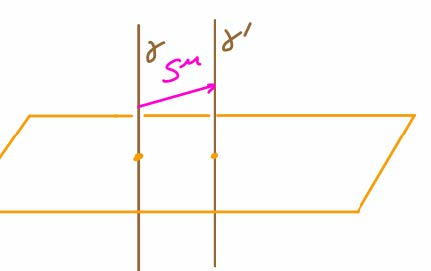
\includegraphics[width=5cm]{../img/ex-geodesic-deviation.jpg}
\end{figure}
\noindent
You will see a non-vanishing acceleration even though coordinates are constant. 
\end{exercise}

%%%%%%%%%%%%%%LECTURE 10%%%%%%%%%%%%

\section{The minimal coupling principle}

\textsf{Carroll, sec. 4.1}\\

So far, we have only considered the effect of a non-trivial gravitational field, i.e. a curved metric, on the motions of a free particle, basically guided by the WEP ($\subset$ EEP). However, invoking the stronger EEP, we can extend the same logic to more general dynamical quantities. This leads us to the \textbf{minimal coupling principle}:
\[\eta\quad\to\quad g_{\mu\nu}(x)\qquad\pde\mu\quad\to\quad\nabla_\mu\]
Notice that, since $[\nabla_\mu,\nabla_\nu]\sim(\text{Riem})$, there may be ambiguites in presence of higher derivatives. 

This prescription is particularly efficient for \emph{Lagrangian densities} of the form
\[\text{Mink}\quad\mathcal L_\Phi(\Phi,\partial\Phi)\quad\longrightarrow\quad\mathcal L_\Phi(\Phi,\nabla\Phi)\]
where $\Phi$ is the set of all gauge and matter fields and $\partial\Phi$ indicates all first derivatives of these fields (all indices on the l.h.s. and on the r.h.s. are contracted respectively through $\eta_{\mu\nu}$ and $\met\mu\nu$).

For instance, for a real scalar field:
\[\mathcal L_\Phi=-\frac12\partial_\mu\phi\partial^\mu\phi-V(\phi)\quad\longrightarrow\quad\mathcal L_\Phi=-\frac12g^{\mu\nu}\nabla_\mu\phi\nabla_\nu\phi-V(\phi)\]
(notice that in this case $\nabla_\mu\phi$ is the same as $\partial_\mu\phi$, but this notation emphasises the covariance). 

For the EM field:
\[
\begin{cases}\mathcal L_A=-\frac14F_{\mu\nu}F^{\mu\nu}+A_\mu J^\mu\\
F_{\mu\nu}=\partial_\mu A_\nu-\partial_\nu A_\mu
\end{cases}
\quad\longrightarrow\quad
\begin{cases}\mathcal L_A=-\frac14\imet\mu\nu\imet\rho\sigma F_{\mu\rho}F_{\nu\sigma}+A_\mu J^\mu=-\frac14F_{\mu\nu}F^{\mu\nu}+A_\mu J^\mu\\
F_{\mu\nu}=\nabla_\mu A_\nu-\nabla_\nu A_\mu=\partial_\mu A_\nu-\partial_\nu A_\mu\quad(\text{since }\chris\mu\nu\rho=\chris\mu\rho\nu)
\end{cases}\]

Having a scalar Lagrangian density $\mathcal L(x)$ we would like to integrate it over (a portion of) spacetime to get an action. We will see how to do this in the next section. 

\section{Integration over curved spaces}\label{sec:integr-curv-space}

\newcommand{\volelem}[1]{\text{d\emph{vol}}_{#1}}

\textsf{Carroll, sec. 2.10}\\

Having a scalar Lagrangian density $\mathcal L(x)$ we would like to integrate it over (a portion of) spacetime to get an action. In this section we will see how to do this. 

First of all, the naivest guess $\int\de^4x\,\lag(x)$ does not work. Indeed, in GR there is no ``canonical'' preferred choice of coordinates and then the spac-time \emph{volume element} $\de^4x$ is ambiguous, being coordinate dependent:
\[\de^4\tilde x=\de^4x\,\left\vert\det\pder{\tilde x^\mu}{x^\nu}\right\vert\]
So, we should identify, in a \emph{coordinate-independent way} a volume element $\volelem4$ to integrate over our space-time. 

In an $n$-dimensional metric space there is natural choice of coordinate independent volume element
\begin{equation}\label{eqn:vol-elem}\boxed{
\volelem n\equiv\de^nx\sqrt{\vert\det g\vert}\equiv\de^n\sqrt{\vert g\vert}
}\end{equation}
where $\det g(x)=\det(\met\mu\nu)$. Indeed, $\tmet\mu\nu=\pder{x^\rho}{\hat x^\mu}\pder{x^\sigma}{\hat x^\nu}\met\rho\sigma$ and then $\det\tilde g(\tilde x)=\left[\det(\pder x{\tilde x})\right]^2\det g(x)$ and
\[\de\widetilde{\text{\emph{vol}}}_n(\tilde x)=\de^n\tilde x\sqrt{\vert\det \tilde g(\tilde x)\vert}=\de^n x\sqrt{\vert\det  g( x)\vert}=\volelem n(x)\]
Notice that if $\met\mu\nu=\delta_{\mu\nu},\eta_{\mu\nu}$ (Euclidean and Minkowskian) then $\volelem n=\de^n x$. Instead, if $\de s^2\vert_{\mathbb E_3}=\de^r+r^2(\de\theta^2+\sin^2\theta\de\phi^2)$ the volume element becomes the usual volume form $\volelem{\mathbb E_3}=\de r\de\theta\de\phi\,r^2\sin\theta$. Therefore eq.~\eqref{eqn:vol-elem} is consistent with usual volume elements in the flat spaces. 

Given canonical volume element eq.~\eqref{eqn:vol-elem}, we can define in an unambiguous and coordinate independent way the integral of any scalar function $f(x)$:
\[\int\de^nx\,\sqrt{\vert\det g\vert}f(x)\]

Notice that the above integral really makes sense if $f(x)$ has support on the coordinate patch. For more general cases, if $ M$ is covered by a set of patches $U_\alpha$, the actual definition of integral of $f$ over $ M$ is obtained by ``weighted'' contributions from different patches by a so-called ``partition of unity''.\footnote{See \cite{Nakahara:2003aa} sec. 5.5 for a detailed description of this statement.} For our purposes, this subtlety will be irrelevant and we will just write
\[I=\int_M\de^nx\,\sqrt{\vert\det g\vert}f(x)\]

For the integration by parts following formula is useful:
\begin{equation}\boxed{
\nabla_\mu V^\mu=\frac1{\sqrt{\vert g\vert}}\pde\mu(\sqrt{\vert g\vert}V^\mu)
}\end{equation}
Using this we obtain the formula for the integration by parts:
\begin{equation}\boxed{\begin{split}
\int_M\de^nx\,\sqrt{\vert\det g\vert}\nabla_\mu V^\mu f(x)
&=\int_M\de^nx\,\pde\mu(\sqrt{\vert\det g\vert}V^\mu) f(x)\\
&=-\int_M\de^nx\,\sqrt{\vert\det g\vert} V^\mu \nabla_\mu f(x)+\text{boundary terms}
\end{split}}\end{equation}

Take any (top) $n$-form in $n$-dimensional manifold\footnote{Note the absence of the factor $1/n!$ when $\mu$ label is omitted.}
\[\omega=\frac1{n!}\omega_{\mu_1\dots\mu_n}\de x^{\mu_1}\wedge\dots\wedge\de x^{\mu_n}
\equiv\omega_{1\dots n}\de x^{1}\wedge\dots\wedge\de x^{n}\]
Under a change of coordinates we have
\[\tilde\omega_{1\dots n}=\pder{x^{\mu_1}}{\tilde x^1}\dots\pder{x^{\mu_n}}{\tilde x^n}\omega_{\mu_1\dots\mu_n}(x)=\det(\pder{x^\mu}{\tilde x^\nu})\omega_{1\dots n}(x)\]
If we fix an orientation on the manifold, so that $\det(\pder{x^\mu}{\tilde x^\nu})>0$, also $\diff nx\omega_{1\dots n}(x)$ is well defined. Hence, the natural definition of integral of a top form $\omega_{(n)}$ over an oriented manifold $M$ is 
\[\int_M\omega\equiv\int_M\diff nx\omega_{1\dots n}(x)\]







\end{document}